% SPDX-License-Identifier: LPPL-1.3c
% Copyright (C) 2026 Christophe Jorssen
% Author and Current Maintainer: Christophe Jorssen <christophe.jorssen@gmail.com>
% LPPL maintenance status: maintained
% This file is part of luafemm. See LICENSE and LICENSES.md for its terms.
\section{A tutorial: charged bodies and ideal capacitors}
\label{sec:tutorial-electric-classics}

Kamil's next lesson concerns Gauss's law. A point charge is useful, but it does
not show how the field behaves inside an extended distribution. He would like
to compare a uniformly charged ball with a charged spherical shell, and then
repeat the experiment with an infinite cylinder. Finally he needs the three
classical capacitors, including a quantitative potential graph.

These models use their exact symmetry solutions. No triangular mesh is needed.
The sphere is three dimensional; the cylinder extends to infinity perpendicular
to the page; the plates extend to infinity in both tangent directions. Each
picture contains one such model, with a homogeneous linear permittivity.
The shaded volume charge is prescribed in an insulating body: it is not a
metal in electrostatic equilibrium.

\luafemmexamplebegin{electric-classics}
\subsection{A ball with a uniform volume charge}
Kamil selects |model=charged sphere|, a radius of one centimetre, and a volume
charge density of $3\times10^{-7}\,\mathrm{C/m^3}$. The geometry pic reads that
same radius. It introduces no second physical object and requires no solve
command. Drawing it first lets the field remain visible over its pale fill.

\begin{codeexample}[width=0pt]
\begin{tikzpicture}[femm/electrostatic={model=charged sphere,
    radius=1,volume charge density=3e-7,name=lesson ball,
    xmin=-2,xmax=2,ymin=-2,ymax=2}]
  \pic {femm electric geometry};
  \pic[femm/electric={levels={.6,.9,1.2,1.5}}] {femm equipotentials};
  \pic {femm electric field};
  \draw[densely dotted,femm/electric profile={name=ball radius,samples=121}]
    (0,0)--(2,0) node[right] {$r$};
  \node[above left] at (0,1) {$\rho$};
\end{tikzpicture}
\end{codeexample}

Inside the ball $E_r=\rho r/(3\epsilon)$, so the field vanishes at the centre
and increases linearly. Outside it decreases as $1/r^2$. The radial lines are
straight in both regions: their appearance alone cannot reveal this change.
A profile will do that. Here $r=x$ on the measurement segment, and |abscissa=x|
will label the horizontal axis in centimetres. Field values remain in V/m.

\subsection{Move the charge to the surface}
For the same total charge Kamil needs $\sigma=\rho R/3=10^{-9}\,\mathrm{C/m^2}$.
He changes the distribution and its density. The outer field is unchanged,
but the hollow interior now has zero field. No line should enter it.

\begin{codeexample}[width=0pt]
\begin{tikzpicture}[femm/electrostatic={model=charged sphere,
    radius=1,charge distribution=surface,surface charge density=1e-9,
    name=lesson shell,xmin=-2,xmax=2,ymin=-2,ymax=2}]
  \pic {femm electric geometry};
  \pic[femm/electric={levels={.6,.9}}] {femm equipotentials};
  \pic {femm electric field};
  \path[femm/electric profile={name=shell radius,samples=121}] (0,0)--(2,0);
  \node at (0,0) {$\mathbf E=\mathbf 0$};
  \node[above left] at (0,1) {$\sigma$};
\end{tikzpicture}
\end{codeexample}

\begin{codeexample}[width=0pt]
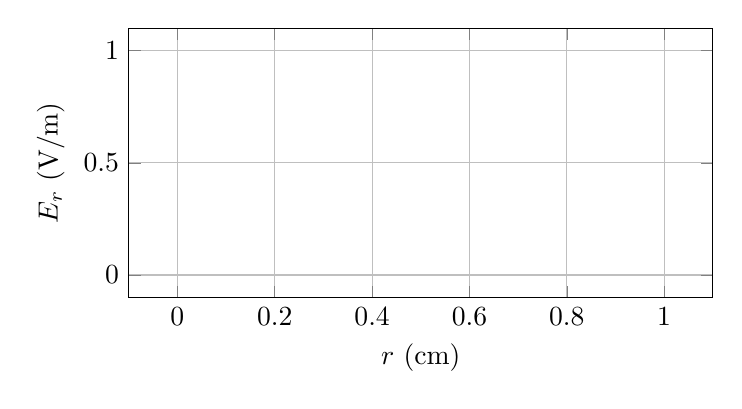
\begin{tikzpicture}
\begin{axis}[width=9cm,height=5cm,no markers,grid=major,
  xlabel={$r$ (cm)},ylabel={$E_r$ (V/m)},legend style={at={(.5,1.03)},anchor=south,legend columns=2}]
  \femmelectricplot[profile=ball radius,component=Ex,abscissa=x,
    plot options={blue!70!black,thick}]
  \addlegendentry{Volume charge}
  \femmelectricplot[profile=shell radius,component=Ex,abscissa=x,
    plot options={red!70!black,dashed,thick}]
  \addlegendentry{Surface charge}
\end{axis}
\end{tikzpicture}
\end{codeexample}

At $r=R$ the shell has two limiting field values. The profile adds both limits
and a gap between them; PGFPlots does not join them by a slanted segment. This
happens even if the original sampling points miss the surface. Increasing
|samples| improves the smooth portions, not the existence of the jump.
The potential, in contrast, is continuous:

\begin{codeexample}[width=0pt]
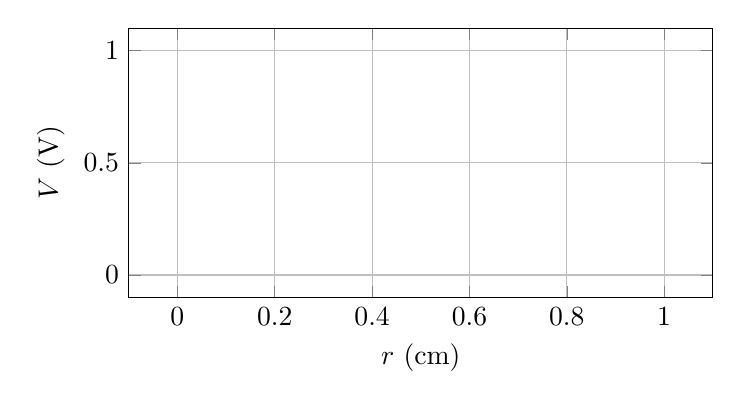
\begin{tikzpicture}
\begin{axis}[width=9cm,height=5cm,no markers,grid=major,
  xlabel={$r$ (cm)},ylabel={$V$ (V)},legend style={at={(.5,1.03)},anchor=south,legend columns=2}]
  \femmelectricplot[profile=ball radius,component=V,abscissa=x,
    plot options={blue!70!black,thick}]
  \addlegendentry{Volume charge}
  \femmelectricplot[profile=shell radius,component=V,abscissa=x,
    plot options={red!70!black,dashed,thick}]
  \addlegendentry{Surface charge}
\end{axis}
\end{tikzpicture}
\end{codeexample}

The flat inner potential of the shell fills a whole disk. It is not a unique
contour curve, so Kamil does not request that constant value as an equipotential
line. Its value is nevertheless present in the graph.

\subsection{A cylinder needs a finite reference radius}
A circular section can describe quite different three-dimensional objects.
Kamil now uses |model=charged cylinder| for an infinite cylinder. Its exterior
field decreases as $1/r$, and its logarithmic potential cannot be set to zero
at infinity. He explicitly chooses |reference radius=2|: $V=0$ at $r=2$ cm.
For the solid cylinder he uses $\rho=2\times10^{-7}\,\mathrm{C/m^3}$; its surface
counterpart has the same charge per length when $\sigma=\rho R/2=10^{-9}\,\mathrm{C/m^2}$.
A style collects their common physical and drawing settings.

\begin{codeexample}[setup code]
\tikzset{lesson cylinder/.style={femm/electrostatic={model=charged cylinder,
  radius=1,reference radius=2,xmin=-2,xmax=2,ymin=-2,ymax=2}}}
\end{codeexample}

\begin{codeexample}[width=0pt]
\begin{tikzpicture}[lesson cylinder,
    femm/electrostatic={volume charge density=2e-7,name=lesson cylinder}]
  \pic {femm electric geometry};
  \pic[femm/electric={levels={.2,.5,.9,1.2}}] {femm equipotentials};
  \pic {femm electric field};
  \path[femm/electric profile={name=cylinder radius,samples=121}]
    (0,0)--(2,0);
\end{tikzpicture}
\begin{tikzpicture}[lesson cylinder,
    femm/electrostatic={charge distribution=surface,
      surface charge density=1e-9,name=lesson cylinder shell}]
  \pic {femm electric geometry};
  \pic[femm/electric={levels={.2,.5}}] {femm equipotentials};
  \pic {femm electric field};
  \path[femm/electric profile={name=cylinder shell radius,samples=121}]
    (0,0)--(2,0);
\end{tikzpicture}
\end{codeexample}

\begin{codeexample}[width=0pt]
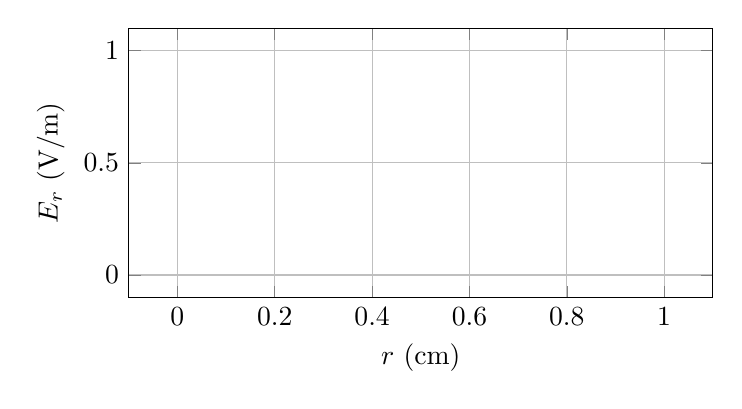
\begin{tikzpicture}
\begin{axis}[width=9cm,height=5cm,no markers,grid=major,
  xlabel={$r$ (cm)},ylabel={$E_r$ (V/m)},legend style={at={(.5,1.03)},anchor=south,legend columns=2}]
  \femmelectricplot[profile=cylinder radius,component=Ex,abscissa=x,
    plot options={blue!70!black,thick}]
  \addlegendentry{Volume charge}
  \femmelectricplot[profile=cylinder shell radius,component=Ex,abscissa=x,
    plot options={red!70!black,dashed,thick}]
  \addlegendentry{Surface charge}
\end{axis}
\end{tikzpicture}
\end{codeexample}

Changing only |reference potential| shifts every potential by the same amount.
It does not change the field or the source charge. The integral result is
available without integrating the plotted curve:

\begin{codeexample}[width=0pt]
$Q=\femmelectricvalue[model=lesson ball,quantity=charge]\,\mathrm C$,\qquad
$\lambda=\femmelectricvalue[model=lesson cylinder,
  quantity=charge per length]\,\mathrm{C/m}$.
\end{codeexample}
\luafemmexampleend{electric-classics}

\luafemmexamplebegin{electric-capacitors}
\subsection{Two plates at prescribed potentials}
Kamil's final set of figures concerns capacitors. Instead of prescribing a
charge density, he prescribes the signed voltage. For the plates,
|normal angle=90| makes the field vertical. With $U=100$ V, the lower plate is
at 100 V and the upper plate is at zero. The separation is one centimetre.
The visible plate span is deliberately wider than the field window: the
physical plates are infinite and there is no edge field.

\begin{codeexample}[width=0pt]
\begin{tikzpicture}[femm/electrostatic={model=parallel plate capacitor,
    separation=1,normal angle=90,voltage=100,name=lesson plates,
    xmin=-2,xmax=2,ymin=-1,ymax=1}]
  \pic[femm/electric={plate span=4.4}] {femm electric geometry};
  \pic[femm/electric={lines per charge=9}] {femm electric field};
  \pic[femm/electric={levels={20,40,60,80}}] {femm equipotentials};
  \node[below] at (0,-.5) {$100\,\mathrm V$};
  \node[above] at (0,.5) {$0\,\mathrm V$};
  \path[femm/electric profile={name=plate normal,samples=121}]
    (0,-1)--(0,1);
\end{tikzpicture}
\end{codeexample}

The measurement contour follows the physical normal, so |abscissa=y| gives
its signed position. The potential changes linearly between the plates and
is flat outside, whereas the field graph has two jumps.

\begin{codeexample}[width=0pt]
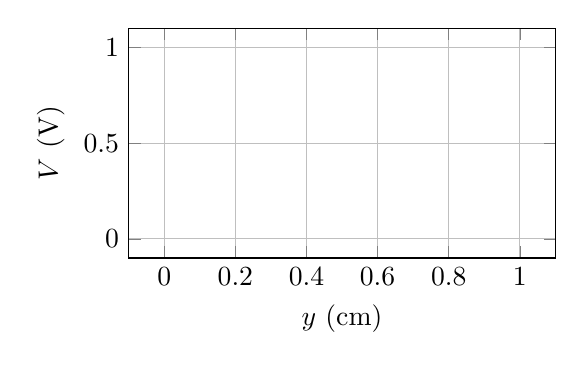
\begin{tikzpicture}
\begin{axis}[width=7cm,height=4.5cm,no markers,grid=major,
  xlabel={$y$ (cm)},ylabel={$V$ (V)}]
  \femmelectricplot[profile=plate normal,component=V,abscissa=y,
    plot options={blue!70!black,thick}]
\end{axis}
\end{tikzpicture}
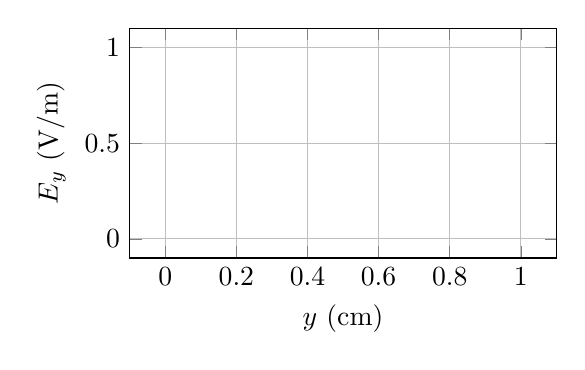
\begin{tikzpicture}
\begin{axis}[width=7cm,height=4.5cm,no markers,grid=major,
  xlabel={$y$ (cm)},ylabel={$E_y$ (V/m)}]
  \femmelectricplot[profile=plate normal,component=Ey,abscissa=y,
    plot options={red!70!black,thick}]
\end{axis}
\end{tikzpicture}
\end{codeexample}

The field is constant between the plates and zero outside. The zero exterior
field is part of this ideal infinite capacitor, not a numerical boundary
condition on the picture window. Reversing |voltage| reverses the arrows;
changing TikZ's |rotate| rotates only the view.

\subsection{The same annulus, two different capacitors}
The next two pictures have identical electrode radii. One is a transverse
section of infinite coaxial cylinders; the other is a central section through
concentric spheres. Both enforce 100 V on the inner electrode and zero on the
outer electrode. The geometrical pic fills the inner conductor, so Kamil draws
it before the field. He samples along a radius that crosses both electrodes.

\begin{codeexample}[setup code]
\tikzset{lesson capacitor/.style={femm/electrostatic={
  inner radius=.7,outer radius=1.4,voltage=100,
  xmin=-1.6,xmax=1.6,ymin=-1.6,ymax=1.6}}}
\end{codeexample}

\begin{codeexample}[width=0pt]
\begin{tikzpicture}[lesson capacitor,
    femm/electrostatic={model=cylindrical capacitor,name=lesson coax}]
  \pic {femm electric geometry};
  \pic {femm electric field};
  \pic[femm/electric={levels={20,40,60,80}}] {femm equipotentials};
  \node at (0,0) {$100\,\mathrm V$};
  \path[femm/electric profile={name=coax radius,samples=161}] (0,0)--(1.6,0);
\end{tikzpicture}
\begin{tikzpicture}[lesson capacitor,
    femm/electrostatic={model=spherical capacitor,name=lesson spherical}]
  \pic {femm electric geometry};
  \pic {femm electric field};
  \pic[femm/electric={levels={20,40,60,80}}] {femm equipotentials};
  \node at (0,0) {$100\,\mathrm V$};
  \path[femm/electric profile={name=spherical radius,samples=161}]
    (0,0)--(1.6,0);
\end{tikzpicture}
\end{codeexample}

The different equipotential spacing becomes particularly clear in a graph.
Using the existing profiles prevents the axes from accidentally describing
a different pair of radii or a different voltage.

\begin{codeexample}[width=0pt]
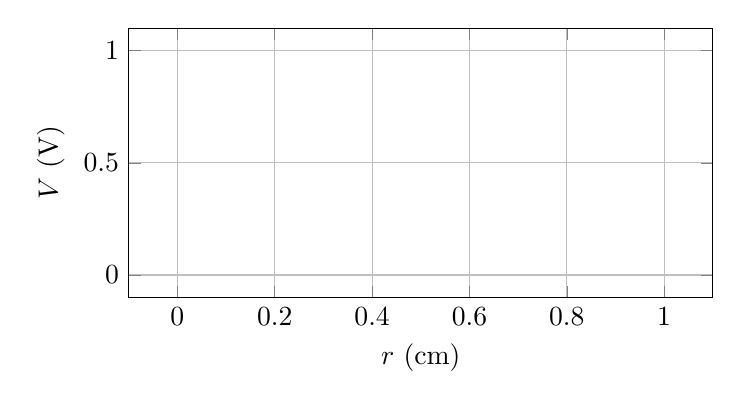
\begin{tikzpicture}
\begin{axis}[width=9cm,height=5cm,no markers,grid=major,
  xlabel={$r$ (cm)},ylabel={$V$ (V)},legend style={at={(.5,1.03)},anchor=south,legend columns=2}]
  \femmelectricplot[profile=coax radius,component=V,abscissa=x,
    plot options={blue!70!black,thick}]
  \addlegendentry{Cylindrical}
  \femmelectricplot[profile=spherical radius,component=V,abscissa=x,
    plot options={red!70!black,dashed,thick}]
  \addlegendentry{Spherical}
\end{axis}
\end{tikzpicture}
\end{codeexample}

\begin{codeexample}[width=0pt]
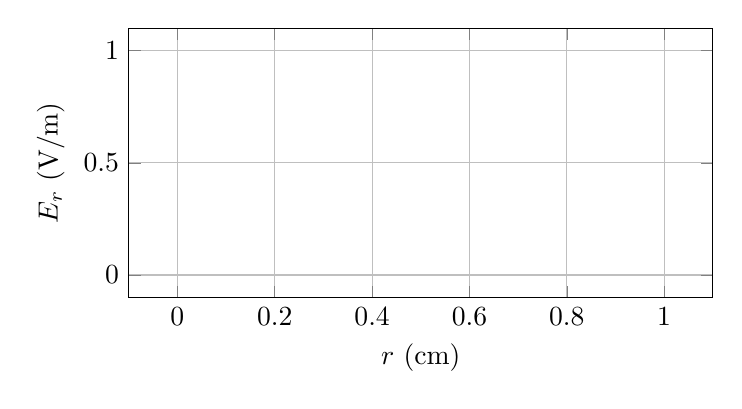
\begin{tikzpicture}
\begin{axis}[width=9cm,height=5cm,no markers,grid=major,
  xlabel={$r$ (cm)},ylabel={$E_r$ (V/m)},legend style={at={(.5,1.03)},anchor=south,legend columns=2}]
  \femmelectricplot[profile=coax radius,component=Ex,abscissa=x,
    plot options={blue!70!black,thick}]
  \addlegendentry{Cylindrical}
  \femmelectricplot[profile=spherical radius,component=Ex,abscissa=x,
    plot options={red!70!black,dashed,thick}]
  \addlegendentry{Spherical}
\end{axis}
\end{tikzpicture}
\end{codeexample}

Both graphs include the constant-potential, zero-field regions inside and
outside the capacitor. No interpolation is drawn through a field jump at an
electrode. The displayed lines have equal angular spacing; their density in
this section is not a quantitative measure of three-dimensional flux.

\subsection{Capacitance and a second view}
An infinite capacitor has no finite total capacitance. Kamil therefore asks
for capacitance per area for the plates and per length for the coaxial model.
The spherical model has a finite total capacitance. The interface rejects a
quantity with the wrong normalization instead of inventing a length or an area.

\begin{codeexample}[width=0pt]
$C/A=\femmelectricvalue[model=lesson plates,
  quantity=capacitance per area]\,\mathrm{F/m^2}$,\quad
$C/L=\femmelectricvalue[model=lesson coax,
  quantity=capacitance per length]\,\mathrm{F/m}$.
\par
$C=\femmelectricvalue[model=lesson spherical,
  quantity=capacitance]\,\mathrm F$,\quad
$W=\femmelectricvalue[model=lesson spherical,quantity=energy]\,\mathrm J$.
\end{codeexample}

A saved model also supplies another view. Its geometry and physical sources
are immutable: Kamil supplies only the snapshot name, the drawing options,
and the seed contour. The latter selects five rays without changing any charge.
For a snapshot with nondefault |length unit| or |relative permittivity|, repeat
those two values when restoring it.

\begin{codeexample}[width=0pt]
\begin{tikzpicture}[femm/electrostatic={snapshot=lesson spherical},rotate=15,
  femm electric conductor/.append style={fill=gray!20},
  femm electric field/.append style={draw=green!45!blue}]
  \pic {femm electric geometry};
  \draw[gray,densely dotted,femm/electric seeds={samples=5}]
    (.9,-.35)--(.9,.35);
  \pic {femm electric field};
\end{tikzpicture}
\end{codeexample}

For a final figure Kamil increases |contour resolution| if the equipotentials
look polygonal, and |samples| if a smooth profile looks coarse. Neither setting
changes the analytical solution. Finite plates, finite cylinder ends and
dielectric interfaces require a different physical model, not more samples.
\luafemmexampleend{electric-capacitors}
